\documentclass{beamer}

\usepackage[british]{babel}
\usepackage{graphicx,hyperref,ru,url}
\usepackage{listings}
\usepackage{fontspec}
\usefonttheme[onlymath]{serif}
\usepackage{xeCJK}
\usepackage[backend=biber]{biblatex}
\bibliography{./ref.bib}
%\addbibresource{ref.bib}
\usepackage{indentfirst}
\usepackage{longtable}
\usepackage{graphicx}
\usepackage{float}
%\usepackage{picins}
\usepackage{rotating}
\usepackage{subfigure}
\usepackage{tabu}
\usepackage{amsmath}
\usepackage{amssymb}
\usepackage{setspace}
\usepackage{amsfonts}
\usepackage{appendix}
\usepackage{listings}
\usepackage{xcolor}
\usepackage{geometry}
\setCJKfamilyfont{cjkhwxk}{STXINGKA.TTF}
\newcommand*{\cjkhwxk}{\CJKfamily{cjkhwxk}}
%\newfontfamily{\consolas}{Consolas}
%\newfontfamily{\monaco}{Monaco}
%\setmonofont[Mapping={}]{Consolas}	%英文引号之类的正常显示,相当于设置英文字体
%\setsansfont{Consolas} %设置英文字体 Monaco, Consolas,  Fantasque Sans Mono
\setmainfont{Times New Roman}
\newfontfamily{\consolas}{YaHeiConsolas.ttf}
\newfontfamily{\monaco}{MONACO.TTF}
\setCJKmainfont{STZHONGS.TTF}
%\setmainfont{MONACO.TTF}
%\setsansfont{MONACO.TTF}
\newcommand{\verylarge}{\fontsize{60pt}{\baselineskip}\selectfont}  
\newcommand{\chuhao}{\fontsize{44.9pt}{\baselineskip}\selectfont}  
\newcommand{\xiaochu}{\fontsize{38.5pt}{\baselineskip}\selectfont}  
\newcommand{\yihao}{\fontsize{27.8pt}{\baselineskip}\selectfont}  
\newcommand{\xiaoyi}{\fontsize{25.7pt}{\baselineskip}\selectfont}  
\newcommand{\erhao}{\fontsize{23.5pt}{\baselineskip}\selectfont}  
\newcommand{\xiaoerhao}{\fontsize{19.3pt}{\baselineskip}\selectfont} 
\newcommand{\sihao}{\fontsize{14pt}{\baselineskip}\selectfont}      % 字号设置  
\newcommand{\xiaosihao}{\fontsize{12pt}{\baselineskip}\selectfont}  % 字号设置  
\newcommand{\wuhao}{\fontsize{10.5pt}{\baselineskip}\selectfont}    % 字号设置  
\newcommand{\xiaowuhao}{\fontsize{9pt}{\baselineskip}\selectfont}   % 字号设置  
\newcommand{\liuhao}{\fontsize{7.875pt}{\baselineskip}\selectfont}  % 字号设置  
\newcommand{\qihao}{\fontsize{5.25pt}{\baselineskip}\selectfont}    % 字号设置 

\definecolor{cred}{rgb}{0.6,0,0}
\definecolor{cgreen}{rgb}{0.25,0.5,0.35}
\definecolor{cpurple}{rgb}{0.5,0,0.35}
\definecolor{cdocblue}{rgb}{0.25,0.35,0.75}
\definecolor{cdark}{rgb}{0.95,1.0,1.0}
\lstset{
	language=R,
	numbers=left,
	numberstyle=\tiny\color{black},
	keywordstyle=\color{cpurple}\consolas,
	commentstyle=\color{cgreen}\consolas,
	stringstyle=\color{cred}\consolas,
	frame=single,
	escapeinside=``,
	xleftmargin=1em,
	xrightmargin=1em, 
	backgroundcolor=\color{cdark},
	aboveskip=1em,
	breaklines=true,
	tabsize=3
} 
% The title of the presentation:
%  - first a short version which is visible at the bottom of each slide;
%  - second the full title shown on the title slide;
\title[Financial Mathematics Presentation]{The Men Behind
  Capital Asset Pricing Model}

% Optional: a subtitle to be dispalyed on the title slide
%\subtitle{Show where you're from}

% The author(s) of the presentation:
%  - again first a short version to be displayed at the bottom;
%  - next the full list of authors, which may include contact information;
\author[****]{
  ****}
% The institute:
%  - to start the name of the university as displayed on the top of each slide
%    this can be adjusted such that you can also create a Dutch version
%  - next the institute information as displayed on the title slide

\institute[\wuhao\fontspec{LHANDW.TTF}Zhejiang University]{\sihao\monaco {School of Mathematical Sciences}}

% Add a date and possibly the name of the event to the slides
%  - again first a short version to be shown at the bottom of each slide
%  - second the full date and event name for the title slide
\date[\today]{
   \today}

\begin{document}

\begin{frame}
  \titlepage
\end{frame}

\begin{frame}
  \frametitle{Outline}

  \tableofcontents
\end{frame}

\section{Introduction}
\begin{frame}{Capital Asset Pricing Model}

\begin{block}{Formula}
	$$
	E[\tilde{r_q}]-r_f=\beta_{qm}(E[\tilde{r_m}]-r_f)
	$$
	where
	\begin{longtable}{ll}
		\hline
		$E[\tilde{r_q}]$ & the expected return on the capital asset\\
		$E[\tilde{r_m}]$& the expected return of the market\\
		$r_f$& the risk-free rate of interest\\
		$\beta_{qm}$&$\dfrac{Cov[\tilde{r_q},\tilde{r_m}]}{Var[\tilde{r_m}]}$\\
		\hline
	\end{longtable}
\end{block}	
\end{frame}


\begin{frame}{Coincidence in Scientific Thought}
	\begin{block}{In the 17th century...}
			\begin{figure}
				\begin{minipage}[t]{0.48\textwidth}
					\centering
					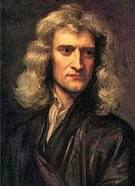
\includegraphics[width=0.6\textwidth]{newton.jpg}\\
					Isaac Newton
				\end{minipage}
				\begin{minipage}[t]{0.48\textwidth}
					\centering
					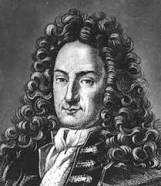
\includegraphics[width=0.7\textwidth]{leibniz.jpg}\\
					Gottfried Leibniz
				\end{minipage}
			\end{figure}
	\end{block}
\end{frame}
\begin{frame}{Coincidence in Scientific Thought}
	\begin{block}{In the 20th century...}
	\begin{figure}
		\begin{minipage}[t]{0.24\textwidth}
			\centering
			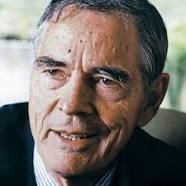
\includegraphics[width=0.9\textwidth]{Jack.jpg}\\
			Jack Treynor(1962)
		\end{minipage}
		\begin{minipage}[t]{0.24\textwidth}
			\centering
			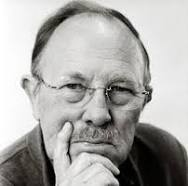
\includegraphics[width=0.9\textwidth]{William.jpg}\\
			\alert{William F.Sharpe(1964)}
		\end{minipage}
		\begin{minipage}[t]{0.24\textwidth}
			\centering
			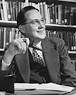
\includegraphics[width=0.9\textwidth]{John.jpg}\\
			John Lintner(1965)
		\end{minipage}
		\begin{minipage}[t]{0.24\textwidth}
			\centering
			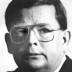
\includegraphics[width=0.9\textwidth]{Jan.jpg}\\
			Jan Mossin(1966)
		\end{minipage}
	\end{figure}
	\end{block}
\end{frame}
\begin{frame}{Coincidence in Scientific Thought}
	\begin{block}{1990 Nobel Memorial Prize in Economics}
		\begin{minipage}[t]{0.3\textwidth}
			\centering
			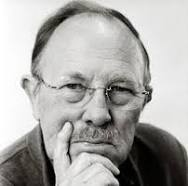
\includegraphics[width=0.9\textwidth]{William.jpg}\\
			\alert{William F.Sharpe}
		\end{minipage}
		\begin{minipage}[t]{0.3\textwidth}
			\centering
			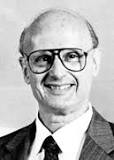
\includegraphics[width=0.9\textwidth]{Markowitz.jpg}\\
			Markowitz
		\end{minipage}
		\begin{minipage}[t]{0.3\textwidth}
			\centering
			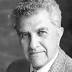
\includegraphics[width=0.9\textwidth]{Merton.jpg}\\
			Merton Miller
		\end{minipage}
	\end{block}
\end{frame}
\begin{frame}{Coincidence in Scientific Thought}
	\chuhao\fontspec{LHANDW.TTF}why?
\end{frame}
\section{Background}
\begin{frame}{Markowitz's work}
	\begin{block}{Portfolio Selection(1952)}
		\begin{figure}
			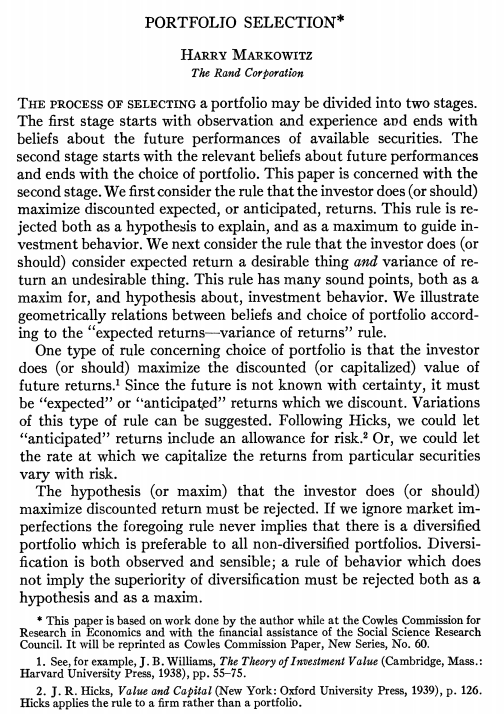
\includegraphics[width=\textwidth]{ps.png}
		\end{figure}
	\end{block}
\end{frame}
\begin{frame}{Markowitz's work}
	\begin{block}{Modern portfolio theory(mean-variance analysis)}
		assembling a portfolio of assets such that \alert{the expected return is maximized }for a given level of risk, defined as variance.
		\begin{figure}
			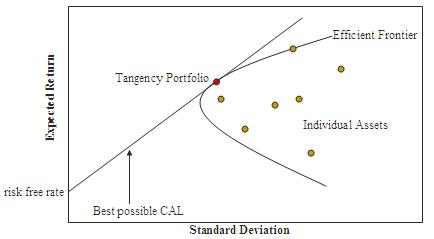
\includegraphics[width=0.8\textwidth]{Markowitz_frontier.jpg}
		\end{figure}
	\end{block}
\end{frame}
\begin{frame}{Franco Modigliani and Merton Miller’s work}
	\begin{itemize}
		\item<2-> “The Cost of Capital, Corporation Finance, and the Theory of Investment.”
		\item<3->the connections between a firm’s capital structure and its cost of capital or discount rate.
		\item<4->\alert{need to} determine the correct discount rate
	\end{itemize}
\end{frame}

\section{Inventors}
\begin{frame}{Jack Treynor(1962)}
	\begin{enumerate}[1.]
		\item<2-> 1958, read Modigliani and Miller's paper
		\item<3-> 1960/1961,``Market Value, Time, and Risk", and show it to John Linter.
		\item<4-> studies economics at MIT
		\item<5-> ``Toward a Theory of Market Value of Risky Assets"\alert{(CAPM)}
		\item<6-> exchange papers with Sharpe
		\item<7-> ``I thought that if Sharpe was going to publish, what's the point of my publishing my paper?" 
	\end{enumerate}
\end{frame}
\begin{frame}{William Sharpe(1964)}
	\begin{enumerate}[1.]
		\item<2-> work at the RAND Corporation and began his PhD studies
		\item<3-> study Markowitz's work
		\item<4-> asked Markowitz for a dissertation topic
		\item<5-> the final chapter of the dissertation\alert{(CAPM)}
		\item<6-> ``Although Harry was not on my committee, he filled a role similar to that of dissertation advisor. My debt to him is truly enormous."
	\end{enumerate}
\end{frame}
\begin{frame}{John Lintner(1965)}
	\begin{enumerate}[1.]
		\item<2-> 1960/1961, Treynor show his work to John Linter.
		\item<3-> 1965, Lintner’s \alert{independent} development of CAPM
		\item<4-> Did Treynor feel that Lintner stole his work?
		\item<5-> How closely do the two papers resemble each other?
		\item<6-> \alert{the most mathematically impressive}
	\end{enumerate}
\end{frame}
\begin{frame}{Jan Mossin(1966)}
	\begin{enumerate}[1.]
		\item<2-> 1966, ``Studies in the Theory of Risk Bearing"\alert{(CAPM)}
		\item<3-> when he began work on CAPM?
		\item<4-> did he know about the other three men's work?
	\end{enumerate}
\end{frame}
\begin{frame}{Comparison}
	\begin{itemize}
		\item Treynor: capital budgeting, cost-of-capital issues
		\item Sharpe: optimum portfolio selection
		\item Linter: the concern of a firm issuing equities.
		\item Mossin: specifying equilibrium conditions in the asset market.
	\end{itemize}
\end{frame}
\section{Conclusion}
\begin{frame}{Why only one Nobel Prize...}
	\alert{The Nobel Prize is not awarded posthumously.}
	\begin{itemize}
		\item<2-> If John Lintner NOT died in 1983 
		\item<3-> If Jan Mossin NOT died in 1987
		\item<4-> If Jack Treynor published his work in 1962
	\end{itemize}
\end{frame}
\begin{frame}{What's more}
	\begin{block}{Black CAPM(zero-beta CAPM)}
		\begin{minipage}{0.3\textwidth}
			\centering
			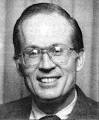
\includegraphics[width=0.9\textwidth]{Fischer.jpg}\\
			Fischer Black
		\end{minipage}
		\begin{minipage}{0.48\textwidth}
			\begin{itemize}
				\item {\color{red}NOT} assume the existence of a riskless asset
				\item more robust!
			\end{itemize}
		\end{minipage}
	\end{block}
\end{frame}
\begin{frame}{Black CAPM(zero-beta CAPM)}
\begin{block}{Formula}
	$$
	E[\tilde{r_q}]-E[\tilde{r}_{zc(m)}]=\beta_{qm}(E[\tilde{r_m}]-E[\tilde{r}_{zc(m)}])
	$$
	where
	\begin{longtable}{ll}
		\hline
		$E[\tilde{r_{zc(m)}}]$& the expected return on the zero-covariance asset\\
		$E[\tilde{r_q}]$ & the expected return on the capital asset\\
		$E[\tilde{r_m}]$& the expected return of the market\\
		%$r_f$& the risk-free rate of interest\\
		$\beta_{qm}$&$\dfrac{Cov[\tilde{r_q},\tilde{r_m}]}{Var[\tilde{r_m}]}$\\
		\hline
	\end{longtable}
\end{block}	
\end{frame}
\begin{frame}[t, allowframebreaks]
\frametitle{References}


\printbibliography
\end{frame}
\begin{frame}
	\chuhao\fontspec{LHANDW.TTF} Thank you!
\end{frame}
\end{document}
